\documentclass{beamer}

%\usepackage{lmodern}
\usepackage[font=scriptsize,skip=0pt,justification=justified,singlelinecheck=false]{caption}
%\usepackage{enumitem}
\usepackage{natbib}
\usepackage{bm}
\usepackage{mathtools}
\usepackage[makeroom]{cancel}


% Insert a Video
\usepackage{multimedia} 

% Using underline
\usepackage{soul}


%remove the icon
\setbeamertemplate{bibliography item}{}

%remove line breaks
\setbeamertemplate{bibliography entry title}{}
\setbeamertemplate{bibliography entry location}{}
\setbeamertemplate{bibliography entry note}{}
% Use number for caption
\setbeamertemplate{caption}[numbered]{}

\newtheorem{mydef}[theorem]{\Large \underline{\textbf{Definisi}}}

\makeatletter
\def\th@mystyle{%
    \normalfont % body font
    \setbeamercolor{block title example}{bg=blue,fg=white}
    \setbeamercolor{block body example}{bg=blue!20,fg=black}
    \def\inserttheoremblockenv{exampleblock}
  }
\makeatother
\theoremstyle{mystyle}
\newtheorem*{remark}{\textbf{Definition}}


% This file is a solution template for:

% - Talk at a conference/colloquium.
% - Talk length is about 20min.
% - Style is ornate.

% Copyright 2004 by Till Tantau <tantau@users.sourceforge.net>.
%
% In principle, this file can be redistributed and/or modified under
% the terms of the GNU Public License, version 2.
%
% However, this file is supposed to be a template to be modified
% for your own needs. For this reason, if you use this file as a
% template and not specifically distribute it as part of a another
% package/program, I grant the extra permission to freely copy and
% modify this file as you see fit and even to delete this copyright
% notice.  


\mode<presentation>
{
%  \usetheme{AnnArbor} % 
%	\usetheme{Frankfurt}
   \usetheme{Madrid}
%	\usetheme{Darmstadt}
  % or ...

%  \setbeamercovered{transparent}
  % or whatever (possibly just delete it)
}


\usepackage[english]{babel}
% or whatever

\usepackage[latin1]{inputenc}
% or whatever

\usepackage{times}
\usepackage[T1]{fontenc}
\usepackage{wasysym}

% Define absolute and norm
\DeclarePairedDelimiter\abs{\lvert}{\rvert}%
\DeclarePairedDelimiter\norm{\lVert}{\rVert}%

% ==============================
%       Redefine emphasize
% ==============================
\let\emph\relax % there's no \RedeclareTextFontCommand
\DeclareTextFontCommand{\emph}{\bfseries\em}


% Swap the definition of \abs* and \norm*, so that \abs
% and \norm resizes the size of the brackets, and the 
% starred version does not.
\makeatletter
\let\oldabs\abs
\def\abs{\@ifstar{\oldabs}{\oldabs*}}
%
\let\oldnorm\norm
\def\norm{\@ifstar{\oldnorm}{\oldnorm*}}
\makeatother

\usepackage{color}
\definecolor{myblue}{rgb}{.8,.8,1}
\usepackage{empheq}
% Or whatever. Note that the encoding and the font should match. If T1
% does not look nice, try deleting the line with the fontenc.

\newlength\mytemplen
\newsavebox\mytempbox

\makeatletter
\newcommand\mybluebox{%
    \@ifnextchar[%]
       {\@mybluebox}%
       {\@mybluebox[0pt]}}

\def\@mybluebox[#1]{%
    \@ifnextchar[%]
       {\@@mybluebox[#1]}%
       {\@@mybluebox[#1][0pt]}}

\def\@@mybluebox[#1][#2]#3{
    \sbox\mytempbox{#3}%
    \mytemplen\ht\mytempbox
    \advance\mytemplen #1\relax
    \ht\mytempbox\mytemplen
    \mytemplen\dp\mytempbox
    \advance\mytemplen #2\relax
    \dp\mytempbox\mytemplen
    \colorbox{myblue}{\hspace{1em}\usebox{\mytempbox}\hspace{1em}}}

\makeatother

\title[Perbedaan Laki-Laki dan Perempuan] % (optional, use only with long paper titles)
{\textbf{Perbedaan Laki-Laki dan Perempuan}\\ \citep{susabda2021konseling}}

%\subtitle
%{\textit{Perbedaan Pria dan Wanita}}

\author[Hendra Bunyamin] % (optional, use only with lots of authors)
{Hendra Bunyamin}
%{F.~Author\inst{1} \and S.~Another\inst{2}} --> original
% - Give the names in the same order as the appear in the paper.
% - Use the \inst{?} command only if the authors have different
%   affiliation.

\institute[ ] % (optional, but mostly needed)
{
%  \inst{1}%
  \hfill \break
  \hfill \break
  \hfill \break
  \large
  Bimbingan Pranikah\\
  GKI Anugerah
%  \and
%  \inst{2}%
%  Department of Theoretical Philosophy\\
%  University of Elsewhere
}
% - Use the \inst command only if there are several affiliations.
% - Keep it simple, no one is interested in your street address.

%\date[CFP 2003] % (optional, should be abbreviation of conference name)
%{Conference on Fabulous Presentations, 2003}
% - Either use conference name or its abbreviation.
% - Not really informative to the audience, more for people (including
%   yourself) who are reading the slides online

\subject{PowerPoint}
% This is only inserted into the PDF information catalog. Can be left
% out. 

% If you have a file called "university-logo-filename.xxx", where xxx
% is a graphic format that can be processed by latex or pdflatex,
% resp., then you can add a logo as follows:

\pgfdeclareimage[height=1.5cm]{university-logo}{logo-gkia-komit}
\logo{\pgfuseimage{university-logo}}


% Delete this, if you do not want the table of contents to pop up at
% the beginning of each subsection:
\AtBeginSection[]
{
  \begin{frame}<beamer>{Outline}
    \tableofcontents[currentsection,currentsection]
  \end{frame}
}


% If you wish to uncover everything in a step-wise fashion, uncomment
% the following command: 

%\beamerdefaultoverlayspecification{<+->}

\begin{document}

\begin{frame}
  \titlepage
\end{frame}

\begin{frame}{The Bunyamins}
	\centering
	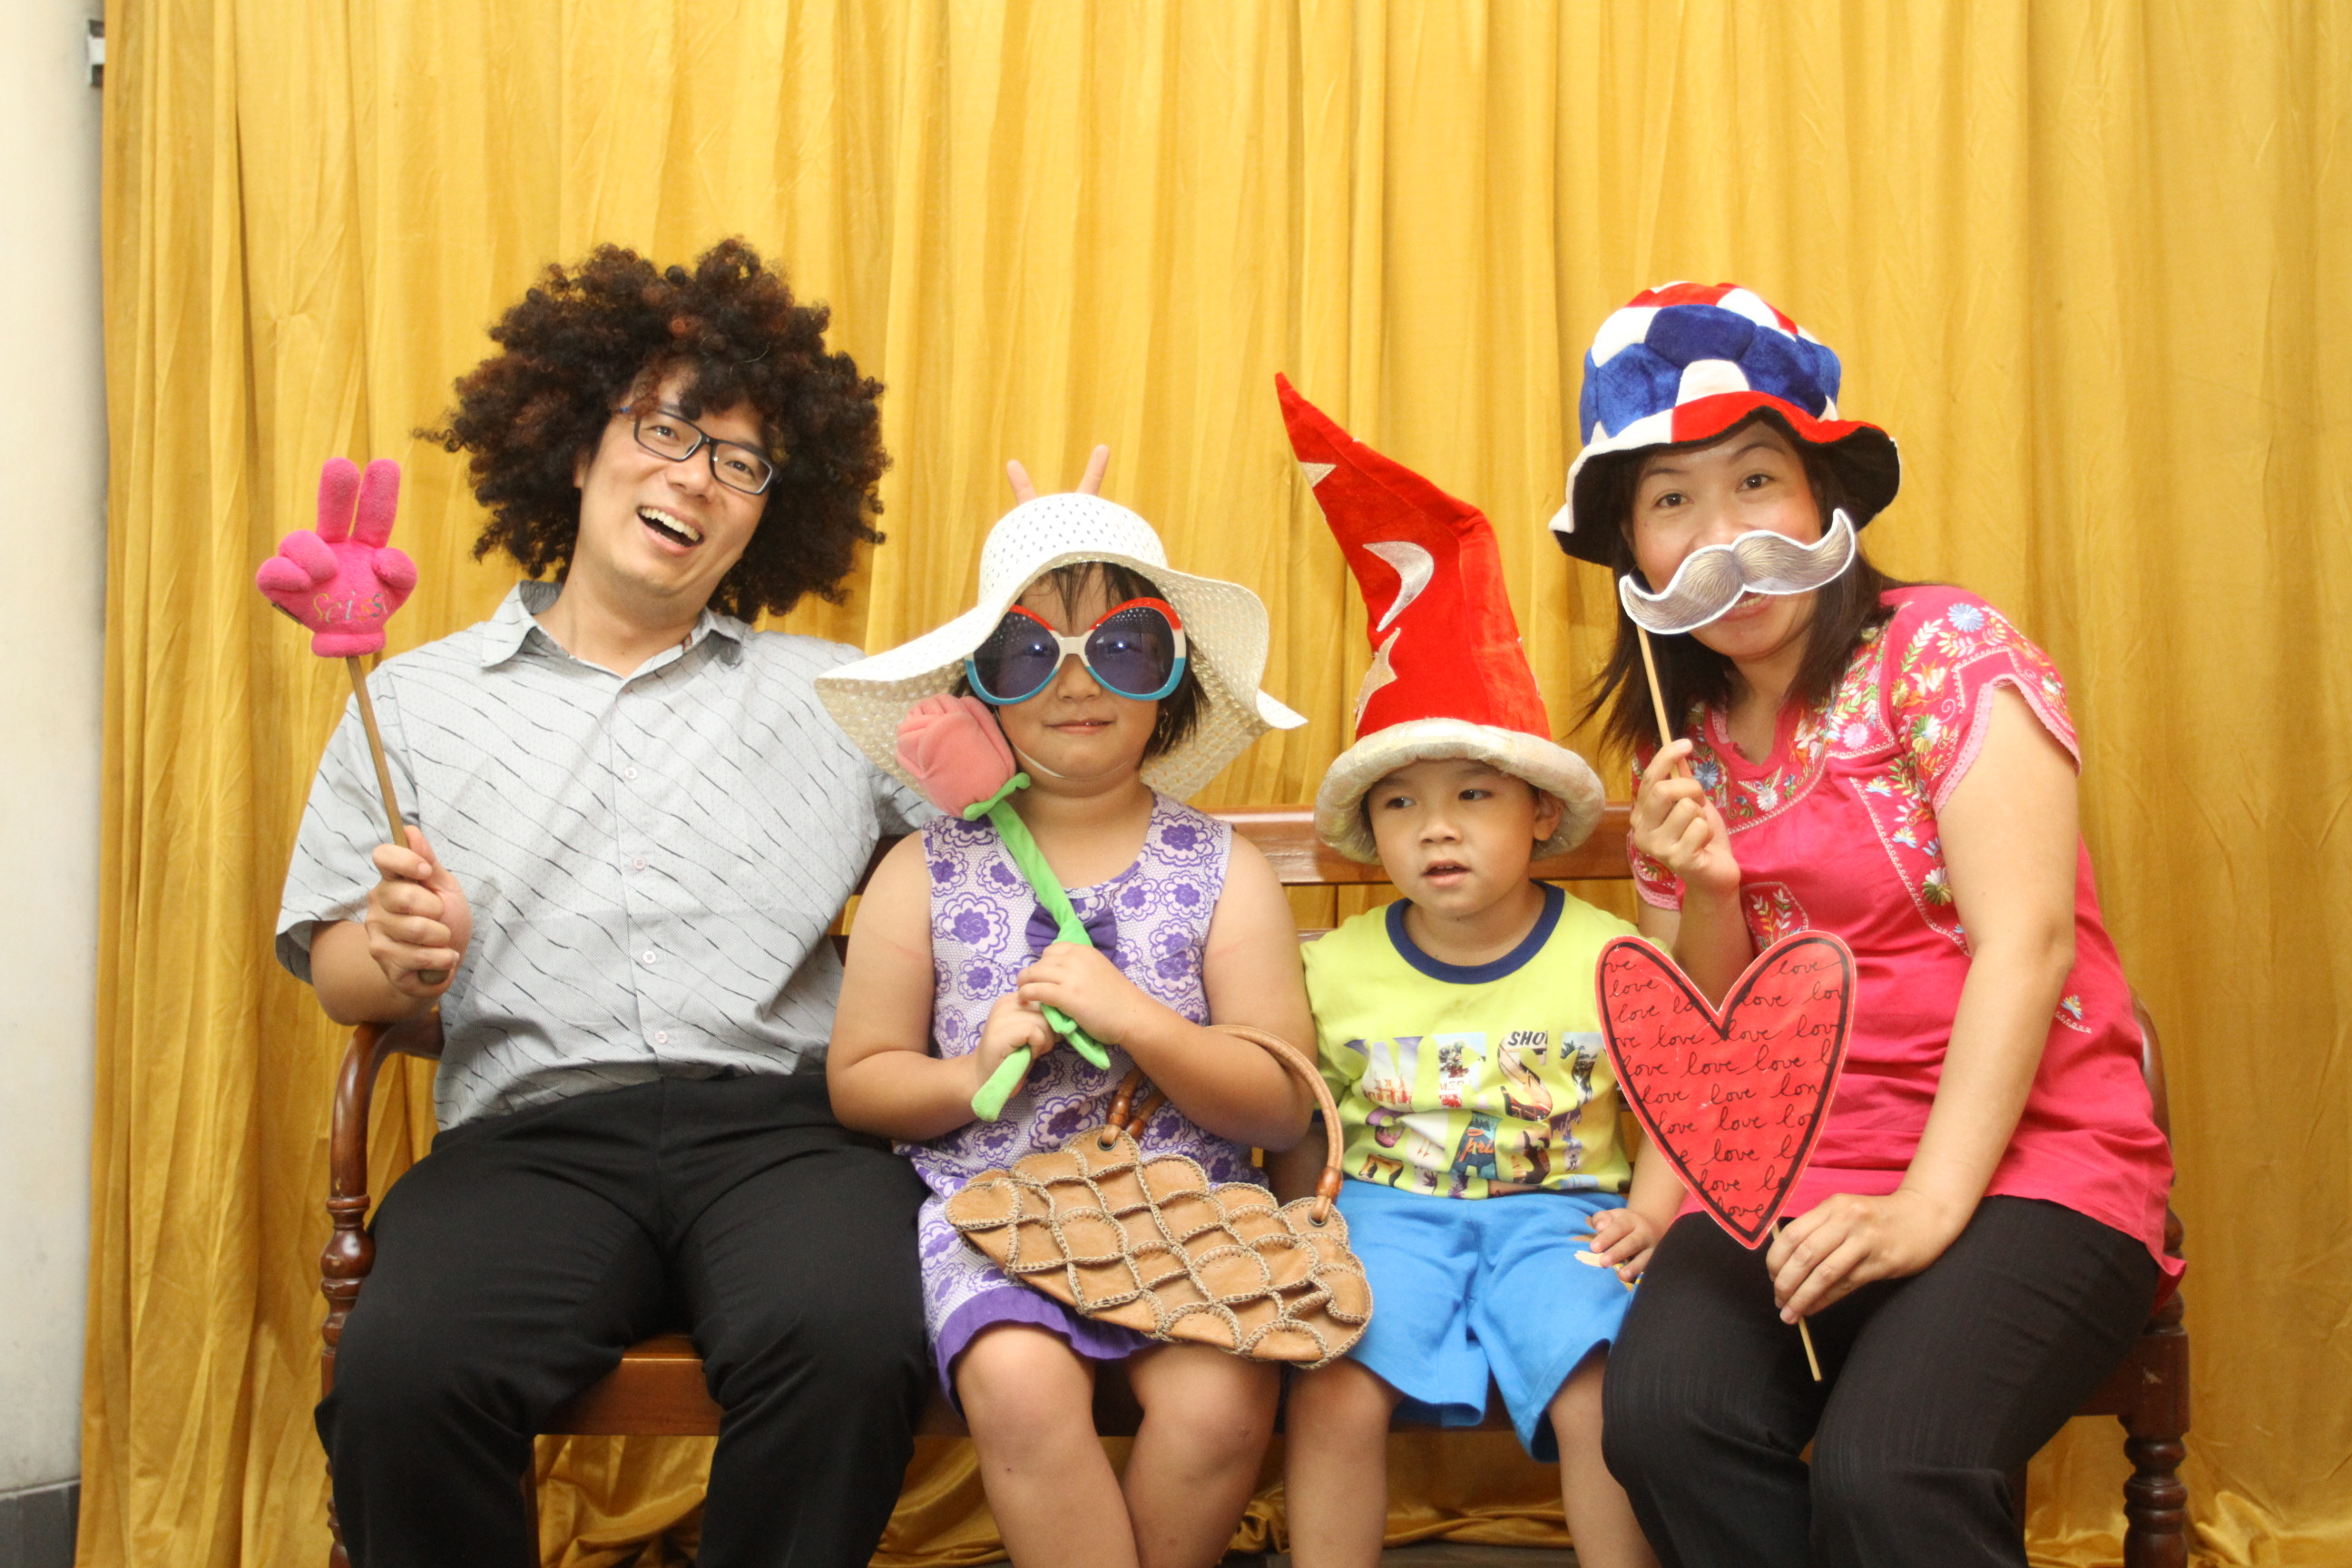
\includegraphics[scale=.125]{family-gullit}
\end{frame}

\begin{frame}{Outline}
  \tableofcontents
  % You might wish to add the option [pausesections]
\end{frame}


% Structuring a talk is a difficult task and the following structure
% may not be suitable. Here are some rules that apply for this
% solution: 

% - Exactly two or three sections (other than the summary).
% - At *most* three subsections per section.
% - Talk about 30s to 2min per frame. So there should be between about
%   15 and 30 frames, all told.

% - A conference audience is likely to know very little of what you
%   are going to talk about. So *simplify*!
% - In a 20min talk, getting the main ideas across is hard
%   enough. Leave out details, even if it means being less precise than
%   you think necessary.
% - If you omit details that are vital to the proof/implementation,
%   just say so once. Everybody will be happy with that.

%\begin{frame}{Make Titles Informative. Use Uppercase Letters.}{Subtitles are optional.}


\section{Apa Kata Alkitab?}
\begin{frame}{Apa kata Alkitab? (1/2)}
 	\emph{Pembacaan Alkitab}
	\begin{itemize}
		\item<2-> \textbf{Kejadian 2:18}\\
		\onslide<3-> TUHAN Allah berfirman: "\textit{Tidak baik, kalau manusia itu seorang diri saja. Aku akan menjadikan penolong baginya, yang sepadan dengan dia.}"
	\end{itemize}
	
	\begin{center} 
		\includegraphics<4->[scale=.25]{my-other-half}
	\end{center}
\end{frame}

\begin{frame}{Apa kata Alkitab? (2/2)}
 	\emph{Pembacaan Alkitab}
	\begin{itemize}
		\item<2-> \textbf{Efesus 5:22-23} \\
		\onslide<3-> \textit{Kasih Kristus adalah dasar hidup suami isteri}
				
		\bigskip
		
		\onslide<4-> Hai isteri, tunduklah kepada suamimu seperti kepada Tuhan, karena suami adalah kepala isteri sama seperti Kristus adalah kepala jemaat. Dialah yang menyelamatkan tubuh.
	\end{itemize}
	\begin{center}
		\includegraphics<5->[scale=.275]{natural-order-in-a-family}	
	\end{center}	
\end{frame}


\section{Natur yang Berbeda}
\begin{frame}{Natur berbeda antara pria dan wanita (1/14)}
	    \textbf{Kejadian 3:16-19}
	    \begin{itemize}
	    	\item<2-> "\textit{Susah payahmu waktu mengandung akan Kubuat sangat banyak; dengan kesakitan engkau akan melahirkan anakmu ...}". \\
	    	\onslide<3-> $\Longrightarrow$ Wanita mendapatkan pemuasan batinnya melalui kesakitan pada saat ia melahirkan anaknya.
	    	\item<4-> "\textit{... engkau akan berahi kepada suamimu dan ia akan berkuasa atasmu.}". \\
	    	\onslide<5-> $\Longrightarrow$ Ketergantungan wanita pada suaminya. \\
	    	\item<6-> "\textit{... terkutuklah tanah karena engkau; dengan bersusah payah engkau akan mencari rezekimu dari tanah seumur hidupmu: ...}" \\
	    	\onslide<7-> $\Longrightarrow$ Pria mengelola bumi dan mendapatkan makanan melalui tenaga yang diperasnya (\textit{lebih membutuhkan kekuatan fisik}).
	    \end{itemize}
%Firman-Nya kepada perempuan itu: "\textit{Susah payahmu waktu mengandung akan Kubuat sangat banyak; dengan kesakitan engkau akan melahirkan anakmu; namun engkau akan berahi kepada suamimu dan ia akan berkuasa atasmu.}" ......, maka \textit{terkutuklah tanah karena engkau; dengan bersusah payah engkau akan mencari rezekimu dari tanah seumur hidupmu: semak duri dan rumput duri yang akan dihasilkannya bagimu, dan tumbuh-tumbuhan di padang akan menjadi makananmu; dengan berpeluh engkau akan mencari makananmu, sampai engkau kembali lagi menjadi tanah, karena dari situlah engkau diambil; sebab engkau debu dan engkau akan kembali menjadi debu.}"
\end{frame}

%\begin{frame}{Natur berbeda antara pria dan wanita (2/22)}
%	\begin{itemize}		
%		\item<2-> Keadaan fisik pria $\Longrightarrow$ pria mengerjakan hal-hal yang memang \textbf{lebih membutuhkan kekuatan fisik}.
%		
%		\bigskip
%
%		\item<3->  Pria mengelola bumi dan mendapatkan makanan melalui tenaga yang diperasnya.
%		
%		\bigskip
%		
%		\item<4-> Wanita mendapatkan pemuasan batinnya melalui kesakitan pada saat ia melahirkan anaknya dan ketergantungannya pada suami.				
%	\end{itemize}
%\end{frame}

\begin{frame}{Natur berbeda antara pria dan wanita (2/14)}
\emph{Yusuf} (\textbf{Matius 1:18-20}): 

	\onslide<2-> Karena Yusuf suaminya, \textit{seorang yang tulus hati dan tidak mau mencemarkan nama isterinya di muka umum, ia bermaksud menceraikannya dengan diam-diam}.
	
	\bigskip
	\onslide<3-> $\Longrightarrow$ Natur yang \textit{yang lebih rasional, cenderung menyelesaikan masalah secara praktis}.

%Kelahiran Yesus Kristus adalah seperti berikut: Pada waktu Maria, ibu-Nya, bertunangan dengan Yusuf, ternyata ia mengandung dari Roh Kudus, sebelum mereka hidup sebagai suami isteri. Karena Yusuf suaminya, \textit{seorang yang tulus hati dan tidak mau mencemarkan nama isterinya di muka umum, ia bermaksud menceraikannya dengan diam-diam}. Tetapi ketika ia mempertimbangkan maksud itu, malaikat Tuhan nampak kepadanya dalam mimpi dan berkata: "Yusuf, anak Daud, janganlah engkau takut mengambil Maria sebagai isterimu, sebab anak yang di dalam kandungannya adalah dari Roh Kudus. 		
\end{frame}

\begin{frame}{Natur berbeda antara pria dan wanita (3/14)}
\emph{Maria} (\textbf{Lukas 1:46-54}): \\
	\onslide<2-> "\textit{Jiwaku memuliakan Tuhan, dan hatiku bergembira karena Allah, Juruselamatku ... Sesungguhnya, mulai dari sekarang segala keturunan akan menyebut aku berbahagia}"
	
	\bigskip
	\onslide<3-> $\Longrightarrow$ Maria bereaksi secara \textit{emosional} atas berita sukacita yang malaikat sampaikan kepadanya.
%Lalu kata Maria: "Jiwaku memuliakan Tuhan, dan hatiku bergembira karena Allah, Juruselamatku sebab Ia telah memperhatikan kerendahan hamba-Nya. Sesungguhnya, mulai dari sekarang segala keturunan akan menyebut aku berbahagia, karena Yang Mahakuasa telah melakukan perbuatan-perbuatan besar kepadaku dan nama-Nya adalah kudus. ......" 	
\end{frame}

%\begin{frame}{Memahami natur yang berbeda antara pria dan wanita (5/22)}
%		\begin{itemize}
%		\item Pria dengan naturnya \textbf{yang lebih rasional cenderung menyelesaikan masalah secara praktis}, berbeda dengan wanita \textbf{yang cenderung lebih mempercayai kerja emosinya}.
%		
%		\bigskip
%		
%		\textbf{Contoh}: Yusuf yang bereaksi secara \textit{rasional} pada saat menemukan Maria, tunangannya yang mengandung 
%
%
%		\bigskip
%		
%		Maria bereaksi secara \textit{emosional} atas berita sukacita yang malaikat sampaikan kepadanya.		
%	\end{itemize}	
%\end{frame}

\begin{frame}{Natur berbeda antara pria dan wanita (4/14)}
	\textbf{Dalam pemenuhan dan pelampiasan kebutuhan seksual}
	
	\bigskip
	\onslide<2-> \emph{Samson} (\textbf{Hakim-Hakim 14-16}):
\begin{itemize}
	\item<3-> "\textit{Di Timna aku melihat seorang gadis Filistin. Tolong, ambillah dia menjadi isteriku.}"
	\item<4-> "\textit{Ambillah dia bagiku, sebab dia kusukai.}"
	\item<5-> \textit{Sesudah itu Simson jatuh cinta kepada seorang perempuan dari lembah Sorek yang namanya Delila}.
\end{itemize}
%	Ia pulang dan memberitahukan kepada ayahnya dan ibunya: "Di Timna aku melihat seorang gadis Filistin. Tolong, ambillah dia menjadi isteriku. Tetapi ayahnya dan ibunya berkata kepadanya: "Tidak adakah di antara anak-anak perempuan sanak saudaramu atau di antara seluruh bangsa kita seorang perempuan, sehingga engkau pergi mengambil isteri dari orang Filistin, orang-orang yang tidak bersunat itu?" Tetapi jawab Simson kepada ayahnya: "Ambillah dia bagiku, sebab dia kusukai." \\
%	$\cdots$ \\
%		$\cdots$ \\
%			$\cdots$ \\
%	Sesudah itu Simson jatuh cinta kepada seorang perempuan dari lembah Sorek yang namanya Delila.
\end{frame}

\begin{frame}{Natur berbeda antara pria dan wanita (5/14)}
	\emph{Daud} \textbf{(2 Samuel 11)}: 
	\begin{itemize}
		\item<2-> "\textit{...tampak kepadanya dari atas sotoh itu seorang perempuan sedang mandi; perempuan itu sangat elok rupanya.}" 
		\item<3-> \textit{Sesudah itu Daud menyuruh orang mengambil dia}.
		\item<4-> lalu \textit{Daud tidur dengan dia}.
	\end{itemize}		
%	...... Sekali peristiwa pada waktu petang, ketika Daud bangun dari tempat pembaringannya, lalu berjalan-jalan di atas sotoh istana, tampak kepadanya dari atas sotoh itu seorang perempuan sedang mandi; perempuan itu sangat elok rupanya. Lalu Daud menyuruh orang bertanya tentang perempuan itu dan orang berkata: "Itu adalah Batsyeba binti Eliam, isteri Uria orang Het itu." Sesudah itu Daud menyuruh orang mengambil dia. Perempuan itu datang kepadanya, lalu \textit{Daud tidur dengan dia}. Perempuan itu baru selesai membersihkan diri dari kenajisannya. Kemudian pulanglah perempuan itu ke rumahnya.	
\end{frame}

\begin{frame}{Natur berbeda antara pria dan wanita (6/14)}
	\emph{Amnon} \textbf{(2 Samuel 13)}:  
	\begin{itemize}
		\item<2-> Absalom bin Daud mempunyai seorang adik perempuan yang cantik, namanya Tamar.
		\item<3-> Hati Amnon sangat tergoda, sehingga ia pura-pura jatuh sakit untuk mendapatkan Tamar.
		\item<4-> ... dipegangnyalah gadis itu dan berkata kepadanya: "\textit{Marilah tidur dengan aku, adikku}."
		\item<5-> Tetapi Amnon tidak mau mendengarkan perkataannya, dan \textit{sebab ia lebih kuat dari padanya, diperkosanyalah dia}, lalu tidur dengan dia.
	\end{itemize}		

	
\end{frame}

\begin{frame}{Natur berbeda antara pria dan wanita (7/14)}
		\onslide<2->\textbf{Contoh-Contoh}: Samson, Daud, Amnon 
		
		\bigskip
		\onslide<3-> $\Longrightarrow$ Pria cenderung \textbf{memenuhi dan melampiaskan kebutuhan seksual secara instan dan semata-mata untuk kepuasan instingnya}, sehingga umumnya mereka tidak dapat memisahkan antara cinta dan seks.
\end{frame}

\begin{frame}{Natur berbeda antara pria dan wanita (8/14)}
\onslide<2-> \emph{Tamar} \textbf{(2 Samuel 13)}: 
\begin{itemize}
	\item<3-> Lalu Lalu Amnon berkata kepadanya: "\textit{Bangunlah, enyahlah!}". 
	\item<4-> Lalu berkatalah gadis itu kepadanya: "\textit{Tidak kakakku, sebab menyuruh aku pergi adalah lebih jahat dari pada apa yang telah kaulakukan kepadaku tadi.}"
	\item<5-> Lalu Tamar menaruh abu di atas kepalanya, mengoyakkan baju kurung yang maha indah yang dipakainya, meletakkan tangannya di atas kepalanya dan pergilah ia sambil meratap dengan nyaring. 
\end{itemize}
\end{frame}


\begin{frame}{Natur berbeda antara pria dan wanita (9/14)}
\onslide<2-> \emph{Lea} \textbf{(Kejadian 30:14-21)}: 

\bigskip
\onslide<3-> Kata Rahel kepada Lea: "\textit{Berilah aku beberapa buah dudaim yang didapat oleh anakmu itu." Jawab Lea kepadanya: "Apakah belum cukup bagimu mengambil suamiku? Sekarang pula mau mengambil lagi buah dudaim anakku?}"

\bigskip

	\onslide<4-> $\Longrightarrow$ \textit{Bagi wanita, hubungan seksual tidak terpisahkan dari keterikatan emosinya}.
	
	\bigskip
	\onslide<5-> $\Longrightarrow$ Hasil empiris juga menemukan bahwa \textit{perzinahan lebih banyak dilakukan oleh pria dibandingkan dengan wanita}. 		
\end{frame}


\begin{frame}{Natur berbeda antara pria dan wanita (10/14)}
	\textbf{Dalam orientasi hidup}
	
	\bigskip
	\onslide<2-> \emph{Yakub} \textbf{(Kejadian 29)}:
	\begin{itemize}
		\item<3-> Yakub cinta kepada Rahel, sebab itu ia berkata: "\textit{Aku mau bekerja padamu tujuh tahun lamanya untuk mendapat Rahel, anakmu yang lebih muda itu.}"
		\item<4-> Jadi bekerjalah Yakub tujuh tahun lamanya untuk mendapat Rahel itu, tetapi yang tujuh tahun itu dianggapnya seperti beberapa hari saja, karena cintanya kepada Rahel. 
		\item<5-> "\textit{... kemudian anakku yang lainpun akan diberikan kepadamu sebagai upah, asal engkau bekerja pula padaku tujuh tahun lagi}".
		\item<6-> Demikianlah ia bekerja pula pada Laban tujuh tahun lagi.
	\end{itemize}			
\end{frame}

\begin{frame}{Natur berbeda antara pria dan wanita (11/14)}
\emph{Pemuda yang kaya} \textbf{(Matius 19)}: 
\begin{itemize}
	\item<2-> Kata orang muda itu kepada-Nya: "\textit{Semuanya itu telah kuturuti, apa lagi yang masih kurang?}"
	\item<3-> Kata Yesus kepadanya: "\textit{Jikalau engkau hendak sempurna, pergilah, juallah segala milikmu dan berikanlah itu kepada orang-orang miskin, maka engkau akan beroleh harta di sorga, kemudian datanglah ke mari dan ikutlah Aku.}"
	\item<4-> Ketika orang muda itu mendengar perkataan itu, pergilah ia dengan sedih, sebab banyak hartanya.
\end{itemize}
\end{frame}

\begin{frame}{Natur berbeda antara pria dan wanita (12/14)}
	
	\textbf{Contoh}: Yakub dan pemuda yang kaya.

	\bigskip
	\onslide<2-> $\Rightarrow$ Pria lebih cenderung \textit{memiliki orientasi hidup pada target dan upaya pencapaiannya} (\textit{target-oriented}). 

\end{frame}


\begin{frame}{Natur berbeda antara pria dan wanita (12/14)}
	\begin{itemize}
		\item<2-> \textbf{Orientasi wanita berubah pada saat kesempatan membina hubungan pribadi itu terbuka} (\textit{relational-oriented}).
		
		\bigskip		
		
		\onslide<3-> \textbf{Contoh}: Rut dan Maria saudara Lazarus (Yohanes 12:1-8).		
	\end{itemize}
\end{frame}

\begin{frame}{Natur berbeda antara pria dan wanita (13/14)}
	\emph{Rut} \textbf{(Rut 1:16-17)}:  

	\bigskip	
	\onslide<2-> Tetapi kata Rut: "\textit{... di mana engkau mati, akupun mati di sana, dan di sanalah aku dikuburkan.}"
	
\end{frame}

\begin{frame}{Natur berbeda antara pria dan wanita (14/14)}
	\emph{Maria saudara Lazarus} \textbf{(Yohanes 12:1-8)}: 

	\bigskip	
	\onslide<2-> ... \textit{Maka Maria mengambil setengah kati minyak narwastu murni yang mahal harganya, lalu meminyaki kaki Yesus dan menyekanya dengan rambutnya; dan bau minyak semerbak di seluruh rumah itu.}
\end{frame}

\section{Peran yang Diberikan Allah}
\begin{frame}{Peran Allah berikan bagi suami dan istri Kristen (1/5)}
	\onslide<2-> \textbf{Sebagai suami}:
	\begin{itemize}
		\item<3-> pria dipanggil untuk menjadi \textbf{kepala keluarga} (Kejadian 2:18, Efesus 5:22-23, 1 Petrus 3:1-7)
	\end{itemize}
	\bigskip
	\onslide<4-> \textbf{Kejadian 2:18}: TUHAN Allah berfirman: "\textit{Tidak baik, kalau manusia itu seorang diri saja. Aku akan menjadikan penolong baginya, yang sepadan dengan dia}."
	
	\bigskip
	\onslide<5-> \textbf{Efesus 5:22-23}: "\textit{Hai isteri, tunduklah kepada suamimu seperti kepada Tuhan, karena suami adalah kepala isteri sama seperti Kristus adalah kepala jemaat. Dialah yang menyelamatkan tubuh}."
\end{frame}

\begin{frame}{Peran Allah berikan bagi suami dan istri Kristen (2/5)}
	\textbf{1 Petrus 3:1-7}: \emph{Hidup bersama suami isteri} \\
	\begin{itemize}
		\item<2-> \textit{hai isteri-isteri, tunduklah kepada suamimu, supaya jika ada di antara mereka yang tidak taat kepada Firman, mereka juga tanpa perkataan dimenangkan oleh kelakuan isterinya, jika mereka melihat, bagaimana murni dan salehnya hidup isteri mereka itu}.
		\item<3-> \textit{Perhiasanmu janganlah secara lahiriah, yaitu dengan mengepang-ngepang rambut, memakai perhiasan emas atau dengan mengenakan pakaian yang indah-indah, tetapi perhiasanmu ialah manusia batiniah yang tersembunyi dengan perhiasan yang tidak binasa yang berasal dari roh yang lemah lembut dan tenteram, yang sangat berharga di mata Allah}.
		\item<4-> \textit{Demikian juga kamu, hai suami-suami, hiduplah bijaksana dengan isterimu, sebagai kaum yang lebih lemah! Hormatilah mereka sebagai teman pewaris dari kasih karunia, yaitu kehidupan, supaya doamu jangan terhalang}.
	\end{itemize}		
\end{frame}

\begin{frame}{Peran Allah berikan bagi suami dan istri Kristen (3/5)}
	\textbf{Sebagai suami}:
	\begin{itemize}
		\item<2-> Sebagai kepala keluarga, ia dipanggil untuk \textit{meneladani Yesus yang menyangkal diri-Nya demi kepentingan orang yang dikasihi-Nya}. 
		
		\bigskip
		\onslide<3-> Prinsip kepemimpinan yang dimulai dengan \textit{memperhambakan dirinya sendiri} (Markus 10:43-44) $\Longrightarrow$ menempatkan pria dalam posisi \textit{leading servant}.											
	\end{itemize}

	\bigskip	
	
	\onslide<4-> \textbf{Markus 10:43-44}: Tidaklah demikian di antara kamu. Barangsiapa ingin menjadi besar di antara kamu, hendaklah ia menjadi \textit{pelayan}mu, dan barangsiapa ingin menjadi yang terkemuka di antara kamu, hendaklah ia menjadi \textit{hamba} untuk semuanya.
\end{frame}

\begin{frame}{Peran Allah berikan bagi suami dan istri Kristen (4/5)}
	\textbf{Sebagai istri}:
	\begin{itemize}
		\item<2-> Sebagai penolong yang sepadan, wanita juga dipanggil untuk meneladani Kristus dalam bentuk \textbf{kerelaan untuk tunduk} (\textit{submissive}) dan menghormati suami. \\
		\onslide<3-> \textbf{Sarah} (1 Petrus 3:1-7) dan \onslide<4-> \textbf{perempuan-perempuan yang saleh di PL} (2 Raja-Raja 4:8-37, Amsal 31:10-31).
	\end{itemize}
	\begin{figure}[ht]
		\centering
		\includegraphics<5->[scale=.25]{perempuan-sunem}
	\end{figure}
\end{frame}

\begin{frame}{Peran Allah berikan bagi suami dan istri Kristen (5/5)}
	\textbf{Sebagai istri}:
	\begin{itemize}		
		\item<2-> Sikap ini hanya dimiliki oleh \textbf{wanita-wanita yang mencintai Tuhan} dan \textbf{rela menyangkal dirinya sendiri}.
		
		\bigskip
		\onslide<3-> Melalui merekalah, Allah berkarya sehingga kehadiran wanita-wanita tersebut \textbf{mengubah dan memperbaharui suami dan seluruh keluarganya} (1 Petrus 3:1-5).		
	\end{itemize}
\end{frame}

\section{Conclusion: Biblical View}
\begin{frame}{Conclusion}
	\begin{itemize}
		\item<2-> Pria sebagai Kepala Keluarga berarti \textit{man has a holy obligation before God to lay down his life for his wife, his children}.
		
		\bigskip		
				
		\item<3-> For a husband, it means that \textit{he has his wife's best interests at heart}, that \textit{he sacrifices his own desires for hers}, that \textit{he puts her first always in his affections}. 
		
		\bigskip		
		
		\item<4-> For a wife, submission in this context means \textit{believing that God is able to work through her husband to accomplish HIS will in her life, to protect her interests}, and \textit{to meet her deepest needs}.
	\end{itemize}
\end{frame}

%\begin{frame}{Blocks}
%\begin{block}{Block Title}
%You can also highlight sections of your presentation in a block, with it's own title
%\end{block}
%\begin{theorem}
%There are separate environments for theorems, examples, definitions and proofs.
%\end{theorem}
%\begin{example}
%Here is an example of an example block.
%\end{example}
%\end{frame}


% All of the following is optional and typically not needed. 
%\appendix
%\section<presentation>*{\appendixname}
%\subsection<presentation>*{For Further Reading}
%
\begin{frame}[allowframebreaks]
  \frametitle<presentation>{\textbf{Referensi}}
    {\footnotesize
    \bibliographystyle{apalike}
    \bibliography{references}
    }    
\end{frame}

%\makeatletter % to change template
%    \setbeamertemplate{headline}[default] % not mandatory, but I though it was better to set it blank
%    \def\beamer@entrycode{\vspace*{-\headheight}} % here is the part we are interested in :)
%\makeatother

%\begin{frame}[plain]
%		\centering
\includegraphics[scale=0.5]{Logo-Maranatha-Untuk-Belakang-02}	
%\end{frame}

\begin{frame}[plain]
		\centering
\includegraphics[scale=1]{thank-you}	
		hendra.bunyamin@gmail.com
\end{frame}


\end{document}


